\begin{wrapfigure}{r}{0.25\textwidth}
    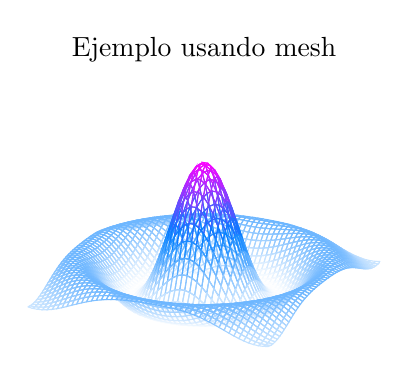
\begin{tikzpicture}
            \begin{axis}
                [
                title=Ejemplo usando mesh,
                hide axis,
                colormap/cool, 
                width=0.5\textwidth]
            \addplot3[mesh,samples=50,domain=-8:8,]{sin(deg(sqrt(x^2+y^2)))/sqrt(x^2+y^2)} ;
            %\addlegendentry{\(\frac{sin(r)}{r}\)}
            \end{axis}
        \end{tikzpicture}
\end{wrapfigure}
\newpage
Este texto esta alrededor de la imagen que hicimos en el penúltimo ejemplo, orientada del lado derecho de nuestro escrito.

\lipsum[1-4]

\begin{wrapfigure}{l}{0.5\textwidth}
\begin{tikzpicture}
\begin{axis}
[
    title={Contour plot, view from top},
    view={0}{90}, width=0.2\textwidth
]
\addplot3[
    contour gnuplot={levels={0.8, 0.4, 0.2, -0.2}}
]
{sin(deg(sqrt(x^2+y^2)))/sqrt(x^2+y^2)};
\end{axis}
\end{tikzpicture}
\end{wrapfigure}
\lipsum[1-6]